\documentclass[189]{pset}

% ================================================================== %
%                                                                    %
%                              Document                              %
%                                                                    %
% ================================================================== %

% ----------------------- Header formatting ------------------------ %

\name{Forest Kobayashi}
\class{Math of Big Data}
\season{Summer}
\prof{Gu}
\assignment{4}
\duedate{05/18/2018}
\dueday{Thursday}
\problems{1, 2}
\acknowledgements{{}, {}}
\onTime{0}

\comments{\textbf{Comments:} Feel free to work with other students,
  but make sure you write up the homework and code on your own (no
  copying homework \textit{or} code; no pair programming). Feel free
  to ask students or instructors for help debugging code or whatever
  else, though.

  The starter files can be found under the Resource tab on course
  website. The graphs for problem 2 generated by the sample solution
  could be found in the corresponding zipfile. These graphs only serve
  as references to your implementation. You should generate your own
  graphs for submission. Please print out all the graphs generated by
  your own code and submit them together with the written part, and
  make sure you upload the code to your Github repository. }

\lfoot{Due Thursday, May 18th 2018}

\begin{document}

% --------------------------- Problem 1 ---------------------------- %

  \section{(Conditioning a Gaussian)}
    \textbf{(Conditioning a Gaussian)} Note that from Murphy page 113.
    ``Equation 4.69 is of such importance in this book that we have
    put a box around it, so you can easily find it.'' That equation is
    important. Read through the proof of the result. Suppose we have a
    distribution over random variables $\vx = (\vx_1, \vx_2)$ that is
    jointly Gaussian with parameters
    \begin{align*}
      \bm{\mu}
      &=
        \begin{bmatrix}
          \bm{\mu}_1 \\
          \bm{\mu}_2
        \end{bmatrix}
      & \bm{\Sigma}
      &=
        \begin{bmatrix}
          \Sigma_{11} & \Sigma_{12} \\
          \Sigma_{21} & \Sigma_{22}
        \end{bmatrix}
    \end{align*}
    where
    \begin{align*}
      \bm{\mu}_1
      &=
        \begin{bmatrix}
          0\\
          0
        \end{bmatrix}
      & \bm{\mu}_2
      &= 5
      & \Sigma_{11}
      &=
        \begin{bmatrix}
          6 & 8 \\
          8 & 13
        \end{bmatrix}
      & \bm{\Sigma}_{21}^\T
      &=
        \begin{bmatrix}
          5 \\
          11
        \end{bmatrix} = \bm{\Sigma}_{12}
      & \Sigma_{22}
      &= [14]
    \end{align*}
    Compute
    \begin{enumerate}
      \item The marginal distribution $p(\vx_1)$.
      \item The marginal distribution $p(\vx_2)$.
      \item The conditional distribution $p(\vx_1 | \vx_2)$
      \item The conditional distribution $p(\vx_2 | \vx_1)$
    \end{enumerate}

  \hrulefill

  \section*{Solution:}
    \begin{enumerate}
      \item We have
        \begin{align*}
          p(\vx_1)
          &= \mc{N}\pn{\vx_1 \mid \bm{\mu}_1, \Sigma_{11}} \\
          &= \frac{1}{\pn{2\pi}^{D/2} \pn{\det\pn{\Sigma_{11}}}^{1/2}}
            \exp\bk{-\frac{1}{2}\pn{\vx - \bm{\mu}}^\T
            \Sigma_{11}^{-1} \pn{\vx - \bm{\mu}}} \\
          &= \frac{1}{2\pi \sqrt{14}} \exp\bk{-\frac{1}{2}\vx^\T
            \frac{1}{14}
            \begin{bmatrix}
              \ph 13 & -8 \\
              - 8 & \ph 6
            \end{bmatrix}\vx } \\
          &= \frac{1}{2\pi \sqrt{14}} \exp\bk{-\frac{1}{28} \pn{13
            x_1^2 - 16x_1x_2 + 6x_2^2}}
        \end{align*}
      \item Looking at the answer key, I'm realizing that that last
        part was unnecessary and that I could have just said
        \begin{align*}
          p(\vx_2)
          &= \mc{N}\pn{\vx_2 \mid \bm{\mu}_2, \Sigma_{22}} \\
          &= \mc{N}\pn{5,14}
        \end{align*}
      \item
        \begin{align*}
          p\pn{\vx_1 \mid \vx_2}
          &= \mc{N}\pn{\vx_1 \mid \bm{\mu}_{1\mid 2}, \Sigma_{1\mid
            2}} \\
          &= \mc{N}\pn{\vx_1 \mid \bm{\mu}_1 + \Sigma_{12}
            \Sigma_{22}^{-1} \pn{\vx_2 - \bm{\mu}_2}, \Sigma_{1\mid
            2}} \\
          &= \mc{N}\pn{\vx_1 \MID \frac{1}{14}
            \begin{bmatrix}
              5 \\
              11
            \end{bmatrix} \pn{\vx_2 - 5}, \Sigma_{11} - \Sigma_{12}
          \Sigma_{22}^{-1} \Sigma_{21}} \\
          &= \mc{N} \pn{
            \begin{bmatrix}
              \frac{5}{14} \\[.5em]
              \frac{11}{14}
            \end{bmatrix} \pn{\vx_2 - 5},
          \begin{bmatrix}
            6 & 8 \\
            8 & 13
          \end{bmatrix}
                - \frac{1}{14}
                \begin{bmatrix}
                  25 & 55 \\
                  55 & 121
                \end{bmatrix}
          }
        \end{align*}
      \item
        \begin{align*}
          p\pn{\vx_2 \mid \vx_1}
          &= \mc{N} \pn{\vx_2 \mid \bm{\mu}_{2\mid 1}, \Sigma_{2\mid
            1}} \\
          &= \mc{N} \pn{\vx_2 \mid 5 +
            \Sigma_{21}\Sigma_{11}^{-1} \pn{\vx_1 - \0}, \Sigma_{2\mid
            1}} \\
          &= \mc{N}\pn{\vx_2 \MID 5 + \frac{1}{14}
            \begin{bmatrix}
              5 & 11
            \end{bmatrix}
                  \begin{bmatrix}
                    \ph 13 & -8 \\
                    -8 & \ph 6
                  \end{bmatrix}
                         \vx_1, [14] - \bk{\frac{171}{14}}} \\
          &= \mc{N}\pn{\vx_2 \MID 5 + \frac{1}{14}
            \begin{bmatrix}
              -23 & 26
            \end{bmatrix} \vx_1, \bk{\frac{25}{14}}} \\
          &= \mc{N}\pn{\vx_2 \MID 5
            \begin{bmatrix}
              -\frac{23}{14} & \frac{13}{7}
            \end{bmatrix} \vx_1, \bk{\frac{25}{14}}} \\
        \end{align*}
    \end{enumerate}

  \clearpage

% --------------------------- Problem 2 ---------------------------- %

  \section{(MNIST)}
    In this problem, we will use the MNIST dataset, a classic in the
    deep learning literature as a toy dataset to test algorithms on,
    to set up a model for logistic regression and softmax regression.
    In the starter code, we have already parsed the data for you.
    However, you might need internet connection to access the data and
    therefore successfully run the starter code.

    The problem is this: we have images of handwritten digits with
    $28\times 28$ pixels in each image, as well as the label of which
    digit $0 \leq \texttt{label} \leq 9$ the written digit corresponds
    to. Given a new image of a handwritten digit, we want to be able
    to predict which digit it is. The format of the data is
    \texttt{label, pix-11, pix-12, pix-13, ...} where \texttt{pix-ij}
    is the pixel in the \texttt{ith} row and \texttt{jth} column.

    \begin{enumerate}
      \item (\textbf{logistic}) Restrict the dataset to only the
        digits with a label of 0 or 1. Implement L2 regularized
        logistic regression as a model to compute $\PP(y=1|\vx)$ for a
        different value of the regularization parameter $\lambda$.
        Plot the learning curve (objective vs. iteration) when using
        Newton's Method \textit{and} gradient descent. Plot the
        accuracy, precision ($p = \PP(y=1 | \hat y=1)$), recall ($r =
        \PP(\hat y=1 | y=1)$), and F1-score ($F1 = 2pr / (p+r)$) for
        different values of $\lambda$ (try at least 10 different
        values including $\lambda = 0$) on the test set and report the
        value of $\lambda$ which maximizes the accuracy on the test
        set. What is your accuracy on the test set for this model?
        Your accuracy should definitely be over 90\%.
      \item (\textbf{softmax}) Now we will use the whole dataset and
        predict the label of each digit using L2 regularized softmax
        regression (multinomial logistic regression). Implement this
        using gradient descent, and plot the accuracy on the test set
        for different values of $\lambda$, the regularization
        parameter. Report the test accuracy for the optimal value of
        $\lambda$ as well as it's learning curve. Your accuracy should
        be over 90\%.
    \end{enumerate}

  \hrulefill

  \section*{Solution:}
    \begin{enumerate}
      \item For the logistic model, we have the same equation as
        previously, just with a regularization term added in:
        \begin{align*}
          \mrm{NLL}(\bm{\theta})
          &= \sum_{i=1}^N \bk{y_i \log\pn{\sigma\pn{\bm{\theta}^T
            \vx_i}} + (1-y^{(i)})\log\pn{1- \sigma\pn{\bm{\theta}^\T
            \vx_i}}} + \lambda \norm{\bm{\theta}}_2^2
        \end{align*}
        \begin{align*}
          \nabla_{\bm{\theta}} \mrm{NLL}\pn{\bm{\theta}}
          &= -\sum_{i=1}^N \bk{y^{(i)}\pn{1-\sigma\pn{\bm{\theta}^\T
            \vx_i}}\vx_i - (1-y^{(i)}) \sigma\pn{\bm{\theta}^\T
            \vx_i}\vx_i} + 2\lambda \bm{\theta} \\
          &= -\sum_{i=1}^N \bk{y^{(i)} - \sigma\pn{\bm{\theta}^\T
            \vx_i}} \vx_i + 2 \lambda \bm{\theta} \\
          &= -X^\T \pn{\vy - \sigma \pn{X\bm{\theta}}} + 2\lambda
            \bm{\theta} \\
          &= X^\T \pn{\sigma \pn{X\bm{\theta}} - \vy} + 2\lambda
            \bm{\theta} \\
        \end{align*}
        the hessian is then
        \begin{align*}
          H
          &= \nabla^2 \mrm{NLL}(\bm{\theta}) \\
          &= \nabla \pn{\sum_{i=1}^N \bk{y^{(i)} -
            \sigma\pn{\bm{\theta}^\T \vx_i}}\vx_i +
            2\lambda\bm{\theta}}^\T \\
          &= \sum_{i=1}^N \bk{\pn{\sigma\pn{\bm{\theta}^\T
            \vx}\vx_i}^\T \vx_i} + 2\lambda I\\
          &= X^\T \diag\pn{\mu_1 \pn{1- \mu_1}, \ldots,
            \mu_n\pn{1-\mu_n}} X + 2\lambda I
        \end{align*}
        where $\mu_i = \sigma\pn{\bm{\theta}^\T\vx_i}$
        \begin{figure}[H]
          \centering
          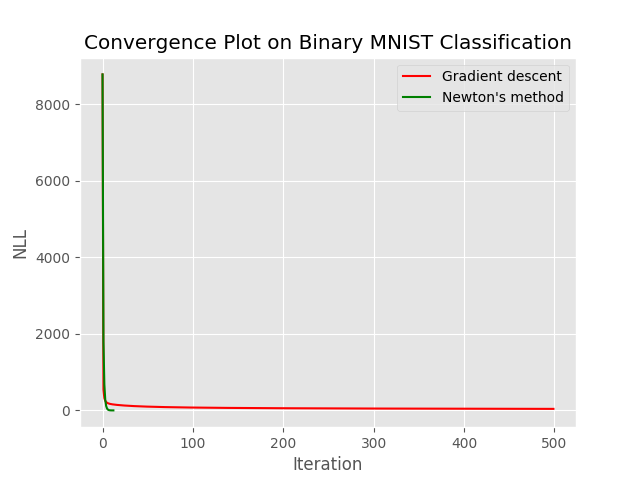
\includegraphics[width=12cm]{hw4pr2a_convergence.png}
        \end{figure}
        \begin{figure}[H]
          \centering
          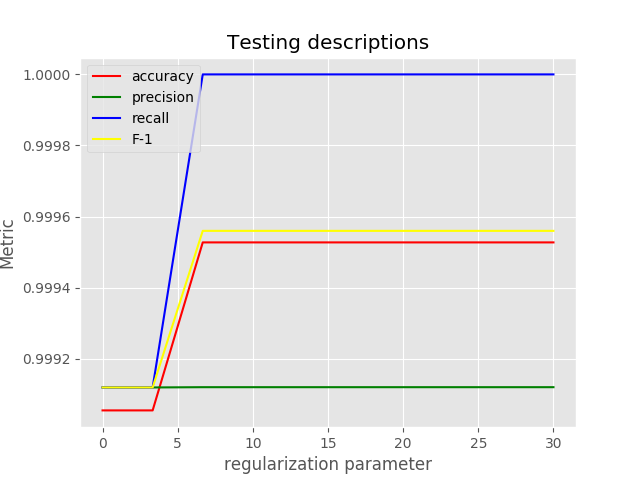
\includegraphics[width=12cm]{hw4pr2a_description.png}
        \end{figure}
      \item We calculate the gradient of the softmax stuff. Our model
        is
        \begin{align*}
          p\pn{y = c \mid \vx, \bW}
          &= \frac{\exp\pn{\bW_c^\T \vx}}{\sum_{c'=1}^C
            \exp\pn{\bW_{c'}^\T \vx}}
        \end{align*}
        let $\mu_{ic} = p\pn{y_i = c \mid \vx_i, \bW} =
        \mc{S}\pn{\bm{\eta_i}}_c$, where $\bm{\eta}_i = \bW^\T \vx_i$.
        Also, let $y_{ic} = \mathbb{I}\pn{y_i = c}$. Let $\vw_C = 0$.
        Hence our one-line log-likelihood equation is
        \begin{align*}
          \mrm{NLL}\pn{\bW}
          &= -\log \pn{\prod_{i=1}^N \prod_{c=1}^C \mu_{ic}^{y_{ic}}}
            + \lambda \norm{\bW}_F \\
          &= \sum_{i=1}^N \sum_{c=1}^C y_{ic} \log\pn{\mu_{ic}} +
            \lambda \tr\pn{\bW^\T \bW}
        \end{align*}
        hence
        \begin{align*}
          \nabla \mrm{NLL}\pn{\bW}
          &= \sum_{i=1}^N \sum_{c=1}^C y_{ic} \pn{1 -
            \mc{S}\pn{\bm{\eta}_i}_c} \vx_i^\T + \lambda \bW \\
          &= X^\T \pn{\bm{\mu} - \bm{y}} + \lambda \bW
        \end{align*}
        \begin{figure}[H]
          \centering
          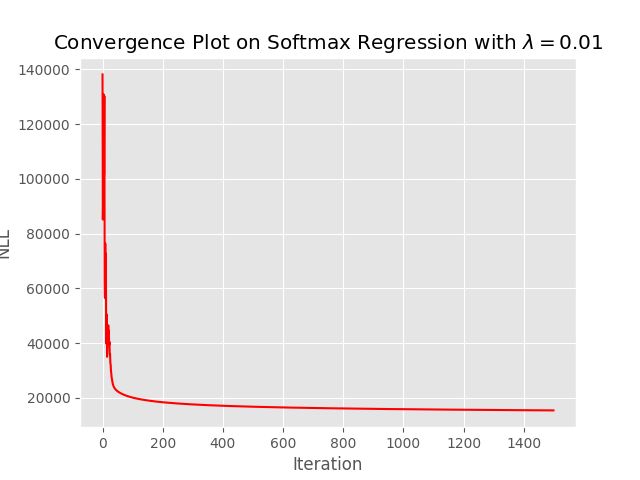
\includegraphics{hw4pr2b_convergence.png}
        \end{figure}
        \begin{figure}[H]
          \centering
          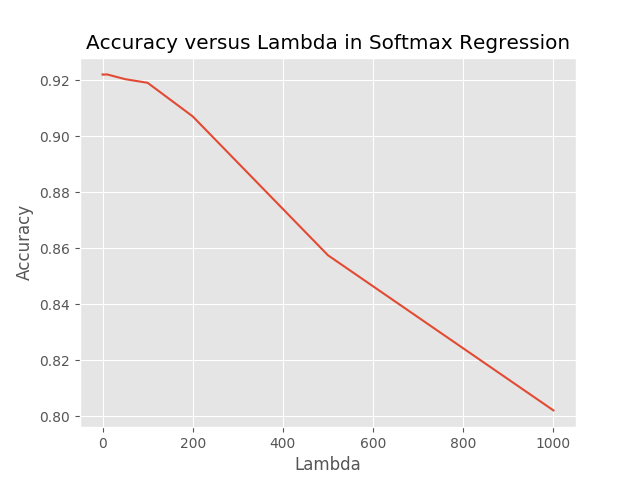
\includegraphics{hw4pr2b_lva.png}
        \end{figure}
    \end{enumerate}
\end{document}
